\documentclass[1p]{elsarticle_modified}
%\bibliographystyle{elsarticle-num}

%\usepackage[colorlinks]{hyperref}
%\usepackage{abbrmath_seonhwa} %\Abb, \Ascr, \Acal ,\Abf, \Afrak
\usepackage{amsfonts}
\usepackage{amssymb}
\usepackage{amsmath}
\usepackage{amsthm}
\usepackage{scalefnt}
\usepackage{amsbsy}
\usepackage{kotex}
\usepackage{caption}
\usepackage{subfig}
\usepackage{color}
\usepackage{graphicx}
\usepackage{xcolor} %% white, black, red, green, blue, cyan, magenta, yellow
\usepackage{float}
\usepackage{setspace}
\usepackage{hyperref}

\usepackage{tikz}
\usetikzlibrary{arrows}

\usepackage{multirow}
\usepackage{array} % fixed length table
\usepackage{hhline}

%%%%%%%%%%%%%%%%%%%%%
\makeatletter
\renewcommand*\env@matrix[1][\arraystretch]{%
	\edef\arraystretch{#1}%
	\hskip -\arraycolsep
	\let\@ifnextchar\new@ifnextchar
	\array{*\c@MaxMatrixCols c}}
\makeatother %https://tex.stackexchange.com/questions/14071/how-can-i-increase-the-line-spacing-in-a-matrix
%%%%%%%%%%%%%%%

\usepackage[normalem]{ulem}

\newcommand{\msout}[1]{\ifmmode\text{\sout{\ensuremath{#1}}}\else\sout{#1}\fi}
%SOURCE: \msout is \stkout macro in https://tex.stackexchange.com/questions/20609/strikeout-in-math-mode

\newcommand{\cancel}[1]{
	\ifmmode
	{\color{red}\msout{#1}}
	\else
	{\color{red}\sout{#1}}
	\fi
}

\newcommand{\add}[1]{
	{\color{blue}\uwave{#1}}
}

\newcommand{\replace}[2]{
	\ifmmode
	{\color{red}\msout{#1}}{\color{blue}\uwave{#2}}
	\else
	{\color{red}\sout{#1}}{\color{blue}\uwave{#2}}
	\fi
}

\newcommand{\Sol}{\mathcal{S}} %segment
\newcommand{\D}{D} %diagram
\newcommand{\A}{\mathcal{A}} %arc


%%%%%%%%%%%%%%%%%%%%%%%%%%%%%5 test

\def\sl{\operatorname{\textup{SL}}(2,\Cbb)}
\def\psl{\operatorname{\textup{PSL}}(2,\Cbb)}
\def\quan{\mkern 1mu \triangleright \mkern 1mu}

\theoremstyle{definition}
\newtheorem{thm}{Theorem}[section]
\newtheorem{prop}[thm]{Proposition}
\newtheorem{lem}[thm]{Lemma}
\newtheorem{ques}[thm]{Question}
\newtheorem{cor}[thm]{Corollary}
\newtheorem{defn}[thm]{Definition}
\newtheorem{exam}[thm]{Example}
\newtheorem{rmk}[thm]{Remark}
\newtheorem{alg}[thm]{Algorithm}

\newcommand{\I}{\sqrt{-1}}
\begin{document}

%\begin{frontmatter}
%
%\title{Boundary parabolic representations of knots up to 8 crossings}
%
%%% Group authors per affiliation:
%\author{Yunhi Cho} 
%\address{Department of Mathematics, University of Seoul, Seoul, Korea}
%\ead{yhcho@uos.ac.kr}
%
%
%\author{Seonhwa Kim} %\fnref{s_kim}}
%\address{Center for Geometry and Physics, Institute for Basic Science, Pohang, 37673, Korea}
%\ead{ryeona17@ibs.re.kr}
%
%\author{Hyuk Kim}
%\address{Department of Mathematical Sciences, Seoul National University, Seoul 08826, Korea}
%\ead{hyukkim@snu.ac.kr}
%
%\author{Seokbeom Yoon}
%\address{Department of Mathematical Sciences, Seoul National University, Seoul, 08826,  Korea}
%\ead{sbyoon15@snu.ac.kr}
%
%\begin{abstract}
%We find all boundary parabolic representation of knots up to 8 crossings.
%
%\end{abstract}
%\begin{keyword}
%    \MSC[2010] 57M25 
%\end{keyword}
%
%\end{frontmatter}

%\linenumbers
%\tableofcontents
%
\newcommand\colored[1]{\textcolor{white}{\rule[-0.35ex]{0.8em}{1.4ex}}\kern-0.8em\color{red} #1}%
%\newcommand\colored[1]{\textcolor{white}{ #1}\kern-2.17ex	\textcolor{white}{ #1}\kern-1.81ex	\textcolor{white}{ #1}\kern-2.15ex\color{red}#1	}

{\Large $\underline{12a_{0246}~(K12a_{0246})}$}

\setlength{\tabcolsep}{10pt}
\renewcommand{\arraystretch}{1.6}
\vspace{1cm}\begin{tabular}{m{100pt}>{\centering\arraybackslash}m{274pt}}
\multirow{5}{120pt}{
	\centering
	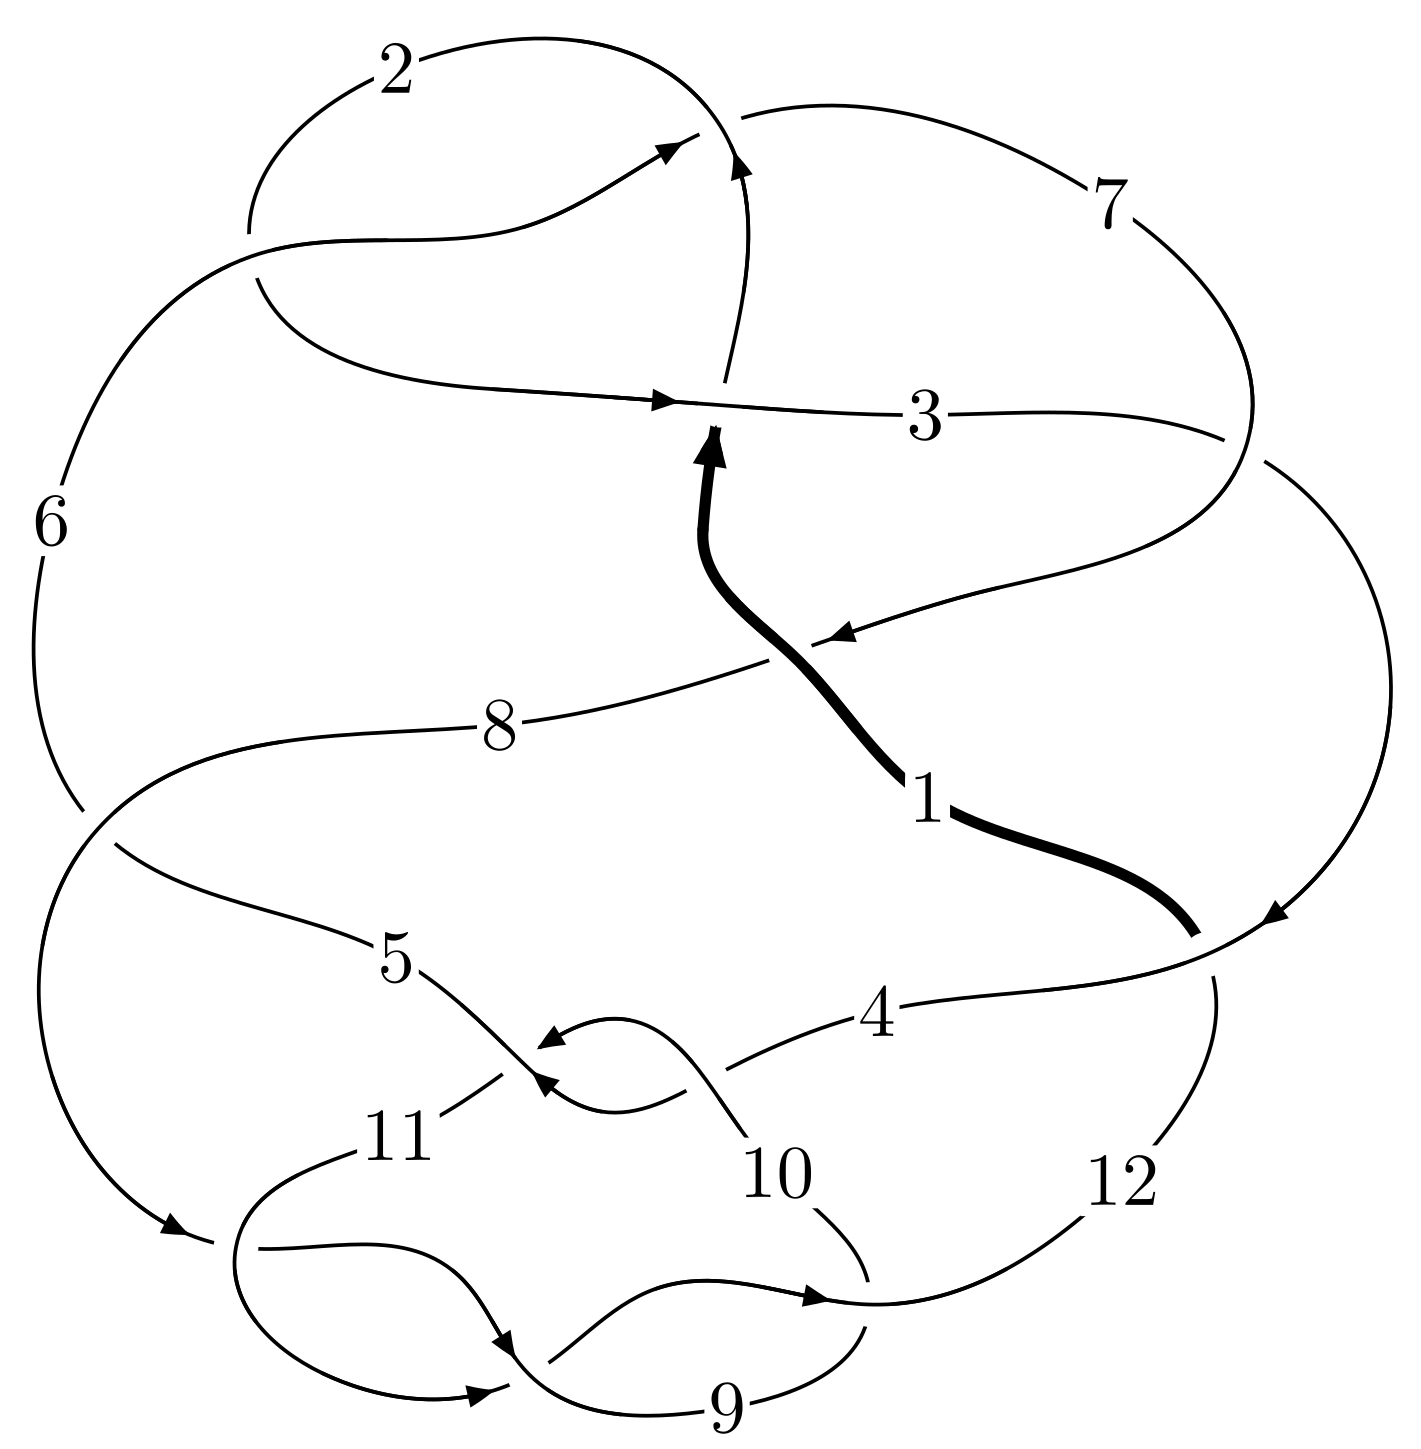
\includegraphics[width=112pt]{../../../GIT/diagram.site/Diagrams/png/1047_12a_0246.png}\\
\ \ \ A knot diagram\footnotemark}&
\allowdisplaybreaks
\textbf{Linearized knot diagam} \\
\cline{2-2}
 &
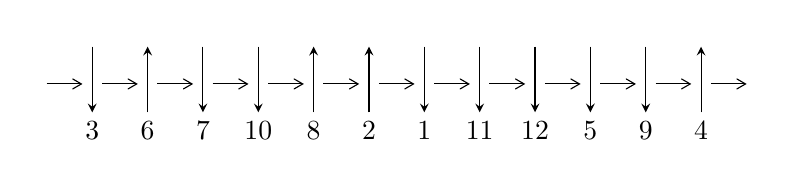
\begin{tikzpicture}[x=20pt, y=17pt]
	% nodes
	\node (C0) at (0, 0) {};
	\node (C1) at (1, 0) {};
	\node (C1U) at (1, +1) {};
	\node (C1D) at (1, -1) {3};

	\node (C2) at (2, 0) {};
	\node (C2U) at (2, +1) {};
	\node (C2D) at (2, -1) {6};

	\node (C3) at (3, 0) {};
	\node (C3U) at (3, +1) {};
	\node (C3D) at (3, -1) {7};

	\node (C4) at (4, 0) {};
	\node (C4U) at (4, +1) {};
	\node (C4D) at (4, -1) {10};

	\node (C5) at (5, 0) {};
	\node (C5U) at (5, +1) {};
	\node (C5D) at (5, -1) {8};

	\node (C6) at (6, 0) {};
	\node (C6U) at (6, +1) {};
	\node (C6D) at (6, -1) {2};

	\node (C7) at (7, 0) {};
	\node (C7U) at (7, +1) {};
	\node (C7D) at (7, -1) {1};

	\node (C8) at (8, 0) {};
	\node (C8U) at (8, +1) {};
	\node (C8D) at (8, -1) {11};

	\node (C9) at (9, 0) {};
	\node (C9U) at (9, +1) {};
	\node (C9D) at (9, -1) {12};

	\node (C10) at (10, 0) {};
	\node (C10U) at (10, +1) {};
	\node (C10D) at (10, -1) {5};

	\node (C11) at (11, 0) {};
	\node (C11U) at (11, +1) {};
	\node (C11D) at (11, -1) {9};

	\node (C12) at (12, 0) {};
	\node (C12U) at (12, +1) {};
	\node (C12D) at (12, -1) {4};
	\node (C13) at (13, 0) {};

	% arrows
	\draw[->,>={angle 60}]
	(C0) edge (C1) (C1) edge (C2) (C2) edge (C3) (C3) edge (C4) (C4) edge (C5) (C5) edge (C6) (C6) edge (C7) (C7) edge (C8) (C8) edge (C9) (C9) edge (C10) (C10) edge (C11) (C11) edge (C12) (C12) edge (C13) ;	\draw[->,>=stealth]
	(C1U) edge (C1D) (C2D) edge (C2U) (C3U) edge (C3D) (C4U) edge (C4D) (C5D) edge (C5U) (C6D) edge (C6U) (C7U) edge (C7D) (C8U) edge (C8D) (C9U) edge (C9D) (C10U) edge (C10D) (C11U) edge (C11D) (C12D) edge (C12U) ;
	\end{tikzpicture} \\
\hhline{~~} \\& 
\textbf{Solving Sequence} \\ \cline{2-2} 
 &
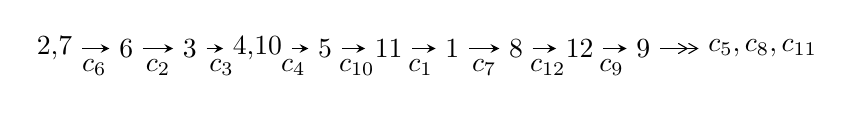
\begin{tikzpicture}[x=23pt, y=7pt]
	% node
	\node (A0) at (-1/8, 0) {2,7};
	\node (A1) at (1, 0) {6};
	\node (A2) at (2, 0) {3};
	\node (A3) at (49/16, 0) {4,10};
	\node (A4) at (33/8, 0) {5};
	\node (A5) at (41/8, 0) {11};
	\node (A6) at (49/8, 0) {1};
	\node (A7) at (57/8, 0) {8};
	\node (A8) at (65/8, 0) {12};
	\node (A9) at (73/8, 0) {9};
	\node (C1) at (1/2, -1) {$c_{6}$};
	\node (C2) at (3/2, -1) {$c_{2}$};
	\node (C3) at (5/2, -1) {$c_{3}$};
	\node (C4) at (29/8, -1) {$c_{4}$};
	\node (C5) at (37/8, -1) {$c_{10}$};
	\node (C6) at (45/8, -1) {$c_{1}$};
	\node (C7) at (53/8, -1) {$c_{7}$};
	\node (C8) at (61/8, -1) {$c_{12}$};
	\node (C9) at (69/8, -1) {$c_{9}$};
	\node (A10) at (11, 0) {$c_{5},c_{8},c_{11}$};

	% edge
	\draw[->,>=stealth]	
	(A0) edge (A1) (A1) edge (A2) (A2) edge (A3) (A3) edge (A4) (A4) edge (A5) (A5) edge (A6) (A6) edge (A7) (A7) edge (A8) (A8) edge (A9) ;
	\draw[->>,>={angle 60}]	
	(A9) edge (A10);
\end{tikzpicture} \\ 

\end{tabular} \\

\footnotetext{
The image of knot diagram is generated by the software ``\textbf{Draw programme}" developed by Andrew Bartholomew(\url{http://www.layer8.co.uk/maths/draw/index.htm\#Running-draw}), where we modified some parts for our purpose(\url{https://github.com/CATsTAILs/LinksPainter}).
}\phantom \\ \newline 
\centering \textbf{Ideals for irreducible components\footnotemark of $X_{\text{par}}$} 
 
\begin{align*}
I^u_{1}&=\langle 
2 u^{84}- u^{83}+\cdots+b+u,\;-2 u^{84}+2 u^{83}+\cdots+a-2,\;u^{86}-2 u^{85}+\cdots+u+1\rangle \\
I^u_{2}&=\langle 
- u^2+b-1,\;u^2+a,\;u^4+u^2- u+1\rangle \\
I^u_{3}&=\langle 
- u^5- u^3+b- u-1,\;a+u+1,\;u^6+u^5+2 u^4+2 u^3+2 u^2+2 u+1\rangle \\
\\
\end{align*}
\raggedright * 3 irreducible components of $\dim_{\mathbb{C}}=0$, with total 96 representations.\\
\footnotetext{All coefficients of polynomials are rational numbers. But the coefficients are sometimes approximated in decimal forms when there is not enough margin.}
\newpage
\renewcommand{\arraystretch}{1}
\centering \section*{I. $I^u_{1}= \langle 2 u^{84}- u^{83}+\cdots+b+u,\;-2 u^{84}+2 u^{83}+\cdots+a-2,\;u^{86}-2 u^{85}+\cdots+u+1 \rangle$}
\flushleft \textbf{(i) Arc colorings}\\
\begin{tabular}{m{7pt} m{180pt} m{7pt} m{180pt} }
\flushright $a_{2}=$&$\begin{pmatrix}0\\u\end{pmatrix}$ \\
\flushright $a_{7}=$&$\begin{pmatrix}1\\0\end{pmatrix}$ \\
\flushright $a_{6}=$&$\begin{pmatrix}1\\u^2\end{pmatrix}$ \\
\flushright $a_{3}=$&$\begin{pmatrix}u\\u^3+u\end{pmatrix}$ \\
\flushright $a_{4}=$&$\begin{pmatrix}- u^3\\u^3+u\end{pmatrix}$ \\
\flushright $a_{10}=$&$\begin{pmatrix}2 u^{84}-2 u^{83}+\cdots-2 u^2+2\\-2 u^{84}+u^{83}+\cdots+2 u^2- u\end{pmatrix}$ \\
\flushright $a_{5}=$&$\begin{pmatrix}u^{16}+3 u^{14}+5 u^{12}+4 u^{10}+3 u^8+2 u^6+2 u^4+1\\u^{18}+4 u^{16}+9 u^{14}+12 u^{12}+11 u^{10}+6 u^8+2 u^6+u^2\end{pmatrix}$ \\
\flushright $a_{11}=$&$\begin{pmatrix}u^{81}- u^{80}+\cdots+u+1\\u^{83}- u^{82}+\cdots- u^3-2 u\end{pmatrix}$ \\
\flushright $a_{1}=$&$\begin{pmatrix}u^3\\u^5+u^3+u\end{pmatrix}$ \\
\flushright $a_{8}=$&$\begin{pmatrix}u^8+u^6+u^4+1\\u^{10}+2 u^8+3 u^6+2 u^4+u^2\end{pmatrix}$ \\
\flushright $a_{12}=$&$\begin{pmatrix}- u^{11}-2 u^9-2 u^7+u^3\\u^{11}+3 u^9+4 u^7+3 u^5+u^3+u\end{pmatrix}$ \\
\flushright $a_{9}=$&$\begin{pmatrix}u^{84}- u^{83}+\cdots+u+2\\- u^{84}+u^{83}+\cdots+u^2- u\end{pmatrix}$\\&\end{tabular}
\flushleft \textbf{(ii) Obstruction class $= -1$}\\~\\
\flushleft \textbf{(iii) Cusp Shapes $= -4 u^{85}+8 u^{84}+\cdots+13 u-2$}\\~\\
\newpage\renewcommand{\arraystretch}{1}
\flushleft \textbf{(iv) u-Polynomials at the component}\newline \\
\begin{tabular}{m{50pt}|m{274pt}}
Crossings & \hspace{64pt}u-Polynomials at each crossing \\
\hline $$\begin{aligned}c_{1}\end{aligned}$$&$\begin{aligned}
&u^{86}+42 u^{85}+\cdots-5 u+1
\end{aligned}$\\
\hline $$\begin{aligned}c_{2},c_{6}\end{aligned}$$&$\begin{aligned}
&u^{86}-2 u^{85}+\cdots+u+1
\end{aligned}$\\
\hline $$\begin{aligned}c_{3}\end{aligned}$$&$\begin{aligned}
&u^{86}+2 u^{85}+\cdots-1288 u+1480
\end{aligned}$\\
\hline $$\begin{aligned}c_{4},c_{10}\end{aligned}$$&$\begin{aligned}
&u^{86}- u^{85}+\cdots-1024 u-1024
\end{aligned}$\\
\hline $$\begin{aligned}c_{5},c_{12}\end{aligned}$$&$\begin{aligned}
&u^{86}+6 u^{85}+\cdots+2399 u+61
\end{aligned}$\\
\hline $$\begin{aligned}c_{7}\end{aligned}$$&$\begin{aligned}
&u^{86}-10 u^{85}+\cdots-1635 u+175
\end{aligned}$\\
\hline $$\begin{aligned}c_{8},c_{9},c_{11}\end{aligned}$$&$\begin{aligned}
&u^{86}-11 u^{85}+\cdots+10 u-1
\end{aligned}$\\
\hline
\end{tabular}\\~\\
\newpage\renewcommand{\arraystretch}{1}
\flushleft \textbf{(v) Riley Polynomials at the component}\newline \\
\begin{tabular}{m{50pt}|m{274pt}}
Crossings & \hspace{64pt}Riley Polynomials at each crossing \\
\hline $$\begin{aligned}c_{1}\end{aligned}$$&$\begin{aligned}
&y^{86}+6 y^{85}+\cdots-53 y+1
\end{aligned}$\\
\hline $$\begin{aligned}c_{2},c_{6}\end{aligned}$$&$\begin{aligned}
&y^{86}+42 y^{85}+\cdots-5 y+1
\end{aligned}$\\
\hline $$\begin{aligned}c_{3}\end{aligned}$$&$\begin{aligned}
&y^{86}-30 y^{85}+\cdots-83985424 y+2190400
\end{aligned}$\\
\hline $$\begin{aligned}c_{4},c_{10}\end{aligned}$$&$\begin{aligned}
&y^{86}-63 y^{85}+\cdots+524288 y+1048576
\end{aligned}$\\
\hline $$\begin{aligned}c_{5},c_{12}\end{aligned}$$&$\begin{aligned}
&y^{86}+78 y^{85}+\cdots-4956101 y+3721
\end{aligned}$\\
\hline $$\begin{aligned}c_{7}\end{aligned}$$&$\begin{aligned}
&y^{86}-6 y^{85}+\cdots-286925 y+30625
\end{aligned}$\\
\hline $$\begin{aligned}c_{8},c_{9},c_{11}\end{aligned}$$&$\begin{aligned}
&y^{86}-89 y^{85}+\cdots-20 y+1
\end{aligned}$\\
\hline
\end{tabular}\\~\\
\newpage\flushleft \textbf{(vi) Complex Volumes and Cusp Shapes}
$$\begin{array}{c|c|c}  
\text{Solutions to }I^u_{1}& \I (\text{vol} + \sqrt{-1}CS) & \text{Cusp shape}\\
 \hline 
\begin{aligned}
u &= -0.288549 + 0.972974 I \\
a &= \phantom{-}1.75493 + 0.78387 I \\
b &= -0.71441 - 1.39976 I\end{aligned}
 & -2.22116 + 0.63715 I & \phantom{-0.000000 } 0 \\ \hline\begin{aligned}
u &= -0.288549 - 0.972974 I \\
a &= \phantom{-}1.75493 - 0.78387 I \\
b &= -0.71441 + 1.39976 I\end{aligned}
 & -2.22116 - 0.63715 I & \phantom{-0.000000 } 0 \\ \hline\begin{aligned}
u &= -0.594363 + 0.827888 I \\
a &= -0.91851 - 1.96253 I \\
b &= \phantom{-}0.014524 + 1.303580 I\end{aligned}
 & -9.68745 + 4.03436 I & \phantom{-0.000000 } 0 \\ \hline\begin{aligned}
u &= -0.594363 - 0.827888 I \\
a &= -0.91851 + 1.96253 I \\
b &= \phantom{-}0.014524 - 1.303580 I\end{aligned}
 & -9.68745 - 4.03436 I & \phantom{-0.000000 } 0 \\ \hline\begin{aligned}
u &= -0.638296 + 0.718655 I \\
a &= \phantom{-}0.621829 + 1.066280 I \\
b &= -1.11853 - 1.20118 I\end{aligned}
 & -9.35445 - 8.83622 I & \phantom{-0.000000 } 0 \\ \hline\begin{aligned}
u &= -0.638296 - 0.718655 I \\
a &= \phantom{-}0.621829 - 1.066280 I \\
b &= -1.11853 + 1.20118 I\end{aligned}
 & -9.35445 + 8.83622 I & \phantom{-0.000000 } 0 \\ \hline\begin{aligned}
u &= -0.555957 + 0.776754 I \\
a &= \phantom{-}1.16780 + 1.58425 I \\
b &= -0.34327 - 1.64073 I\end{aligned}
 & -2.77437 + 0.31938 I & \phantom{-0.000000 } 0 \\ \hline\begin{aligned}
u &= -0.555957 - 0.776754 I \\
a &= \phantom{-}1.16780 - 1.58425 I \\
b &= -0.34327 + 1.64073 I\end{aligned}
 & -2.77437 - 0.31938 I & \phantom{-0.000000 } 0 \\ \hline\begin{aligned}
u &= \phantom{-}0.581383 + 0.747816 I \\
a &= -0.883363 + 0.244616 I \\
b &= -0.160269 + 0.234378 I\end{aligned}
 & -4.82698 + 2.27835 I & -7.05026 + 0. I\phantom{ +0.000000I} \\ \hline\begin{aligned}
u &= \phantom{-}0.581383 - 0.747816 I \\
a &= -0.883363 - 0.244616 I \\
b &= -0.160269 - 0.234378 I\end{aligned}
 & -4.82698 - 2.27835 I & -7.05026 + 0. I\phantom{ +0.000000I}\\
 \hline 
 \end{array}$$\newpage$$\begin{array}{c|c|c}  
\text{Solutions to }I^u_{1}& \I (\text{vol} + \sqrt{-1}CS) & \text{Cusp shape}\\
 \hline 
\begin{aligned}
u &= -0.596508 + 0.722178 I \\
a &= -0.96022 - 1.17170 I \\
b &= \phantom{-}0.89133 + 1.57341 I\end{aligned}
 & -2.57785 - 4.86252 I & -5.77848 + 6.73279 I \\ \hline\begin{aligned}
u &= -0.596508 - 0.722178 I \\
a &= -0.96022 + 1.17170 I \\
b &= \phantom{-}0.89133 - 1.57341 I\end{aligned}
 & -2.57785 + 4.86252 I & -5.77848 - 6.73279 I \\ \hline\begin{aligned}
u &= -0.165912 + 1.053050 I \\
a &= -1.46305 - 1.21359 I \\
b &= \phantom{-}0.58657 + 1.44609 I\end{aligned}
 & -8.18316 + 2.86607 I & \phantom{-0.000000 } 0 \\ \hline\begin{aligned}
u &= -0.165912 - 1.053050 I \\
a &= -1.46305 + 1.21359 I \\
b &= \phantom{-}0.58657 - 1.44609 I\end{aligned}
 & -8.18316 - 2.86607 I & \phantom{-0.000000 } 0 \\ \hline\begin{aligned}
u &= \phantom{-}0.349534 + 1.027830 I \\
a &= -1.12480 + 0.89092 I \\
b &= \phantom{-}0.106873 - 0.233450 I\end{aligned}
 & -4.50001 + 0.99756 I & \phantom{-0.000000 } 0 \\ \hline\begin{aligned}
u &= \phantom{-}0.349534 - 1.027830 I \\
a &= -1.12480 - 0.89092 I \\
b &= \phantom{-}0.106873 + 0.233450 I\end{aligned}
 & -4.50001 - 0.99756 I & \phantom{-0.000000 } 0 \\ \hline\begin{aligned}
u &= \phantom{-}0.472766 + 0.978829 I \\
a &= \phantom{-}0.632946 - 0.143360 I \\
b &= -0.0900200 + 0.0714641 I\end{aligned}
 & -0.31789 + 2.37544 I & \phantom{-0.000000 } 0 \\ \hline\begin{aligned}
u &= \phantom{-}0.472766 - 0.978829 I \\
a &= \phantom{-}0.632946 + 0.143360 I \\
b &= -0.0900200 - 0.0714641 I\end{aligned}
 & -0.31789 - 2.37544 I & \phantom{-0.000000 } 0 \\ \hline\begin{aligned}
u &= -0.409816 + 1.044080 I \\
a &= -2.51537 + 0.29188 I \\
b &= \phantom{-}1.78380 + 1.41570 I\end{aligned}
 & -3.34460 - 3.00265 I & \phantom{-0.000000 } 0 \\ \hline\begin{aligned}
u &= -0.409816 - 1.044080 I \\
a &= -2.51537 - 0.29188 I \\
b &= \phantom{-}1.78380 - 1.41570 I\end{aligned}
 & -3.34460 + 3.00265 I & \phantom{-0.000000 } 0\\
 \hline 
 \end{array}$$\newpage$$\begin{array}{c|c|c}  
\text{Solutions to }I^u_{1}& \I (\text{vol} + \sqrt{-1}CS) & \text{Cusp shape}\\
 \hline 
\begin{aligned}
u &= \phantom{-}0.662896 + 0.554239 I \\
a &= -0.209758 + 0.606442 I \\
b &= \phantom{-}0.607340 + 0.402687 I\end{aligned}
 & -2.86044 + 2.76662 I & -5.58462 - 3.68598 I \\ \hline\begin{aligned}
u &= \phantom{-}0.662896 - 0.554239 I \\
a &= -0.209758 - 0.606442 I \\
b &= \phantom{-}0.607340 - 0.402687 I\end{aligned}
 & -2.86044 - 2.76662 I & -5.58462 + 3.68598 I \\ \hline\begin{aligned}
u &= \phantom{-}0.569259 + 0.995615 I \\
a &= -0.950968 - 0.816360 I \\
b &= \phantom{-}0.354473 - 0.196976 I\end{aligned}
 & -4.15735 + 2.02652 I & \phantom{-0.000000 } 0 \\ \hline\begin{aligned}
u &= \phantom{-}0.569259 - 0.995615 I \\
a &= -0.950968 + 0.816360 I \\
b &= \phantom{-}0.354473 + 0.196976 I\end{aligned}
 & -4.15735 - 2.02652 I & \phantom{-0.000000 } 0 \\ \hline\begin{aligned}
u &= \phantom{-}0.789520 + 0.286900 I \\
a &= \phantom{-}0.055631 + 0.848882 I \\
b &= -3.06816 - 0.09259 I\end{aligned}
 & -11.5254 - 10.8225 I & -8.61250 + 5.48206 I \\ \hline\begin{aligned}
u &= \phantom{-}0.789520 - 0.286900 I \\
a &= \phantom{-}0.055631 - 0.848882 I \\
b &= -3.06816 + 0.09259 I\end{aligned}
 & -11.5254 + 10.8225 I & -8.61250 - 5.48206 I \\ \hline\begin{aligned}
u &= \phantom{-}0.524013 + 1.035860 I \\
a &= \phantom{-}0.017411 + 0.996158 I \\
b &= -0.225482 - 0.283637 I\end{aligned}
 & \phantom{-}0.34446 + 3.37846 I & \phantom{-0.000000 } 0 \\ \hline\begin{aligned}
u &= \phantom{-}0.524013 - 1.035860 I \\
a &= \phantom{-}0.017411 - 0.996158 I \\
b &= -0.225482 + 0.283637 I\end{aligned}
 & \phantom{-}0.34446 - 3.37846 I & \phantom{-0.000000 } 0 \\ \hline\begin{aligned}
u &= -0.286242 + 1.129260 I \\
a &= -0.253145 + 0.710934 I \\
b &= \phantom{-}0.598687 - 0.429451 I\end{aligned}
 & -4.99538 + 0.14999 I & \phantom{-0.000000 } 0 \\ \hline\begin{aligned}
u &= -0.286242 - 1.129260 I \\
a &= -0.253145 - 0.710934 I \\
b &= \phantom{-}0.598687 + 0.429451 I\end{aligned}
 & -4.99538 - 0.14999 I & \phantom{-0.000000 } 0\\
 \hline 
 \end{array}$$\newpage$$\begin{array}{c|c|c}  
\text{Solutions to }I^u_{1}& \I (\text{vol} + \sqrt{-1}CS) & \text{Cusp shape}\\
 \hline 
\begin{aligned}
u &= \phantom{-}0.537821 + 0.631209 I \\
a &= \phantom{-}0.450398 - 0.045646 I \\
b &= \phantom{-}0.001813 - 0.214183 I\end{aligned}
 & \phantom{-}0.69758 + 1.71362 I & \phantom{-}1.48385 - 4.15054 I \\ \hline\begin{aligned}
u &= \phantom{-}0.537821 - 0.631209 I \\
a &= \phantom{-}0.450398 + 0.045646 I \\
b &= \phantom{-}0.001813 + 0.214183 I\end{aligned}
 & \phantom{-}0.69758 - 1.71362 I & \phantom{-}1.48385 + 4.15054 I \\ \hline\begin{aligned}
u &= -0.726874 + 0.393872 I \\
a &= \phantom{-}0.112798 + 0.574879 I \\
b &= \phantom{-}1.17469 + 0.88530 I\end{aligned}
 & -3.62779 + 4.95156 I & -6.26943 - 4.18360 I \\ \hline\begin{aligned}
u &= -0.726874 - 0.393872 I \\
a &= \phantom{-}0.112798 - 0.574879 I \\
b &= \phantom{-}1.17469 - 0.88530 I\end{aligned}
 & -3.62779 - 4.95156 I & -6.26943 + 4.18360 I \\ \hline\begin{aligned}
u &= -0.498379 + 1.066840 I \\
a &= -2.07471 + 1.96310 I \\
b &= \phantom{-}2.57897 + 0.42300 I\end{aligned}
 & -2.71273 - 3.72235 I & \phantom{-0.000000 } 0 \\ \hline\begin{aligned}
u &= -0.498379 - 1.066840 I \\
a &= -2.07471 - 1.96310 I \\
b &= \phantom{-}2.57897 - 0.42300 I\end{aligned}
 & -2.71273 + 3.72235 I & \phantom{-0.000000 } 0 \\ \hline\begin{aligned}
u &= \phantom{-}0.770621 + 0.275590 I \\
a &= -0.157069 - 1.026500 I \\
b &= \phantom{-}2.99026 + 0.32459 I\end{aligned}
 & -4.69326 - 6.52919 I & -6.81472 + 5.27474 I \\ \hline\begin{aligned}
u &= \phantom{-}0.770621 - 0.275590 I \\
a &= -0.157069 + 1.026500 I \\
b &= \phantom{-}2.99026 - 0.32459 I\end{aligned}
 & -4.69326 + 6.52919 I & -6.81472 - 5.27474 I \\ \hline\begin{aligned}
u &= -0.767665 + 0.262811 I \\
a &= -0.492258 + 0.383127 I \\
b &= -0.563795 + 1.146430 I\end{aligned}
 & -7.06528 + 3.78113 I & -8.10408 - 2.38629 I \\ \hline\begin{aligned}
u &= -0.767665 - 0.262811 I \\
a &= -0.492258 - 0.383127 I \\
b &= -0.563795 - 1.146430 I\end{aligned}
 & -7.06528 - 3.78113 I & -8.10408 + 2.38629 I\\
 \hline 
 \end{array}$$\newpage$$\begin{array}{c|c|c}  
\text{Solutions to }I^u_{1}& \I (\text{vol} + \sqrt{-1}CS) & \text{Cusp shape}\\
 \hline 
\begin{aligned}
u &= \phantom{-}0.277554 + 1.162930 I \\
a &= -3.44039 - 1.29200 I \\
b &= \phantom{-}2.31723 - 1.08605 I\end{aligned}
 & -9.10196 - 3.37594 I & \phantom{-0.000000 } 0 \\ \hline\begin{aligned}
u &= \phantom{-}0.277554 - 1.162930 I \\
a &= -3.44039 + 1.29200 I \\
b &= \phantom{-}2.31723 + 1.08605 I\end{aligned}
 & -9.10196 + 3.37594 I & \phantom{-0.000000 } 0 \\ \hline\begin{aligned}
u &= \phantom{-}0.296845 + 1.162430 I \\
a &= \phantom{-}2.88869 + 1.49562 I \\
b &= -2.07890 + 0.99513 I\end{aligned}
 & -9.33402 + 2.30663 I & \phantom{-0.000000 } 0 \\ \hline\begin{aligned}
u &= \phantom{-}0.296845 - 1.162430 I \\
a &= \phantom{-}2.88869 - 1.49562 I \\
b &= -2.07890 - 0.99513 I\end{aligned}
 & -9.33402 - 2.30663 I & \phantom{-0.000000 } 0 \\ \hline\begin{aligned}
u &= -0.287047 + 1.165100 I \\
a &= \phantom{-}0.45506 - 1.42515 I \\
b &= -1.20531 + 0.95369 I\end{aligned}
 & -11.41770 + 0.56506 I & \phantom{-0.000000 } 0 \\ \hline\begin{aligned}
u &= -0.287047 - 1.165100 I \\
a &= \phantom{-}0.45506 + 1.42515 I \\
b &= -1.20531 - 0.95369 I\end{aligned}
 & -11.41770 - 0.56506 I & \phantom{-0.000000 } 0 \\ \hline\begin{aligned}
u &= \phantom{-}0.768626 + 0.218313 I \\
a &= \phantom{-}0.077135 - 1.268350 I \\
b &= \phantom{-}2.17103 + 0.10227 I\end{aligned}
 & -12.50220 + 2.89654 I & -9.84851 - 1.14586 I \\ \hline\begin{aligned}
u &= \phantom{-}0.768626 - 0.218313 I \\
a &= \phantom{-}0.077135 + 1.268350 I \\
b &= \phantom{-}2.17103 - 0.10227 I\end{aligned}
 & -12.50220 - 2.89654 I & -9.84851 + 1.14586 I \\ \hline\begin{aligned}
u &= \phantom{-}0.757922 + 0.251411 I \\
a &= \phantom{-}0.071124 + 1.222860 I \\
b &= -2.56236 - 0.49445 I\end{aligned}
 & -5.06705 - 0.94141 I & -7.86259 - 0.41236 I \\ \hline\begin{aligned}
u &= \phantom{-}0.757922 - 0.251411 I \\
a &= \phantom{-}0.071124 - 1.222860 I \\
b &= -2.56236 + 0.49445 I\end{aligned}
 & -5.06705 + 0.94141 I & -7.86259 + 0.41236 I\\
 \hline 
 \end{array}$$\newpage$$\begin{array}{c|c|c}  
\text{Solutions to }I^u_{1}& \I (\text{vol} + \sqrt{-1}CS) & \text{Cusp shape}\\
 \hline 
\begin{aligned}
u &= \phantom{-}0.262587 + 1.173330 I \\
a &= \phantom{-}3.53054 + 0.94911 I \\
b &= -2.41749 + 1.15092 I\end{aligned}
 & -16.0850 - 7.6716 I & \phantom{-0.000000 } 0 \\ \hline\begin{aligned}
u &= \phantom{-}0.262587 - 1.173330 I \\
a &= \phantom{-}3.53054 - 0.94911 I \\
b &= -2.41749 - 1.15092 I\end{aligned}
 & -16.0850 + 7.6716 I & \phantom{-0.000000 } 0 \\ \hline\begin{aligned}
u &= \phantom{-}0.519924 + 1.085570 I \\
a &= \phantom{-}1.03946 - 1.48640 I \\
b &= -0.148695 + 1.038150 I\end{aligned}
 & -3.28429 + 5.87626 I & \phantom{-0.000000 } 0 \\ \hline\begin{aligned}
u &= \phantom{-}0.519924 - 1.085570 I \\
a &= \phantom{-}1.03946 + 1.48640 I \\
b &= -0.148695 - 1.038150 I\end{aligned}
 & -3.28429 - 5.87626 I & \phantom{-0.000000 } 0 \\ \hline\begin{aligned}
u &= -0.541621 + 1.081200 I \\
a &= \phantom{-}0.68625 - 1.95841 I \\
b &= -1.88134 + 0.43680 I\end{aligned}
 & -0.49878 - 7.28560 I & \phantom{-0.000000 } 0 \\ \hline\begin{aligned}
u &= -0.541621 - 1.081200 I \\
a &= \phantom{-}0.68625 + 1.95841 I \\
b &= -1.88134 - 0.43680 I\end{aligned}
 & -0.49878 + 7.28560 I & \phantom{-0.000000 } 0 \\ \hline\begin{aligned}
u &= -0.432231 + 1.134090 I \\
a &= \phantom{-}2.07510 - 0.96389 I \\
b &= -2.17476 - 0.86834 I\end{aligned}
 & -11.08480 - 3.93749 I & \phantom{-0.000000 } 0 \\ \hline\begin{aligned}
u &= -0.432231 - 1.134090 I \\
a &= \phantom{-}2.07510 + 0.96389 I \\
b &= -2.17476 + 0.86834 I\end{aligned}
 & -11.08480 + 3.93749 I & \phantom{-0.000000 } 0 \\ \hline\begin{aligned}
u &= \phantom{-}0.313991 + 1.175220 I \\
a &= -2.43370 - 1.04010 I \\
b &= \phantom{-}1.75385 - 1.21759 I\end{aligned}
 & -16.7193 + 6.3367 I & \phantom{-0.000000 } 0 \\ \hline\begin{aligned}
u &= \phantom{-}0.313991 - 1.175220 I \\
a &= -2.43370 + 1.04010 I \\
b &= \phantom{-}1.75385 + 1.21759 I\end{aligned}
 & -16.7193 - 6.3367 I & \phantom{-0.000000 } 0\\
 \hline 
 \end{array}$$\newpage$$\begin{array}{c|c|c}  
\text{Solutions to }I^u_{1}& \I (\text{vol} + \sqrt{-1}CS) & \text{Cusp shape}\\
 \hline 
\begin{aligned}
u &= -0.726678 + 0.290250 I \\
a &= \phantom{-}0.272140 - 0.169725 I \\
b &= \phantom{-}0.280985 - 0.574993 I\end{aligned}
 & -0.80863 + 3.09743 I & -0.14695 - 3.21978 I \\ \hline\begin{aligned}
u &= -0.726678 - 0.290250 I \\
a &= \phantom{-}0.272140 + 0.169725 I \\
b &= \phantom{-}0.280985 + 0.574993 I\end{aligned}
 & -0.80863 - 3.09743 I & -0.14695 + 3.21978 I \\ \hline\begin{aligned}
u &= -0.571260 + 1.092910 I \\
a &= \phantom{-}0.24119 + 1.91899 I \\
b &= \phantom{-}1.49187 - 1.07630 I\end{aligned}
 & -5.67694 - 9.90189 I & \phantom{-0.000000 } 0 \\ \hline\begin{aligned}
u &= -0.571260 - 1.092910 I \\
a &= \phantom{-}0.24119 - 1.91899 I \\
b &= \phantom{-}1.49187 + 1.07630 I\end{aligned}
 & -5.67694 + 9.90189 I & \phantom{-0.000000 } 0 \\ \hline\begin{aligned}
u &= \phantom{-}0.590836 + 0.487016 I \\
a &= \phantom{-}0.033582 - 0.610913 I \\
b &= -0.555184 + 0.176196 I\end{aligned}
 & \phantom{-}1.95612 + 1.07254 I & \phantom{-}2.32786 - 4.06564 I \\ \hline\begin{aligned}
u &= \phantom{-}0.590836 - 0.487016 I \\
a &= \phantom{-}0.033582 + 0.610913 I \\
b &= -0.555184 - 0.176196 I\end{aligned}
 & \phantom{-}1.95612 - 1.07254 I & \phantom{-}2.32786 + 4.06564 I \\ \hline\begin{aligned}
u &= -0.651259 + 0.383779 I \\
a &= -0.297043 - 0.580610 I \\
b &= -1.327010 - 0.235305 I\end{aligned}
 & \phantom{-}1.52038 + 2.62568 I & \phantom{-}0.05256 - 5.40036 I \\ \hline\begin{aligned}
u &= -0.651259 - 0.383779 I \\
a &= -0.297043 + 0.580610 I \\
b &= -1.327010 + 0.235305 I\end{aligned}
 & \phantom{-}1.52038 - 2.62568 I & \phantom{-}0.05256 + 5.40036 I \\ \hline\begin{aligned}
u &= -0.546113 + 1.127960 I \\
a &= -0.819362 - 0.114303 I \\
b &= \phantom{-}0.342254 + 0.774577 I\end{aligned}
 & -3.23683 - 7.93121 I & \phantom{-0.000000 } 0 \\ \hline\begin{aligned}
u &= -0.546113 - 1.127960 I \\
a &= -0.819362 + 0.114303 I \\
b &= \phantom{-}0.342254 - 0.774577 I\end{aligned}
 & -3.23683 + 7.93121 I & \phantom{-0.000000 } 0\\
 \hline 
 \end{array}$$\newpage$$\begin{array}{c|c|c}  
\text{Solutions to }I^u_{1}& \I (\text{vol} + \sqrt{-1}CS) & \text{Cusp shape}\\
 \hline 
\begin{aligned}
u &= \phantom{-}0.541262 + 1.146140 I \\
a &= \phantom{-}3.19594 + 2.07479 I \\
b &= -3.56382 + 0.39183 I\end{aligned}
 & -7.67401 + 5.81428 I & \phantom{-0.000000 } 0 \\ \hline\begin{aligned}
u &= \phantom{-}0.541262 - 1.146140 I \\
a &= \phantom{-}3.19594 - 2.07479 I \\
b &= -3.56382 - 0.39183 I\end{aligned}
 & -7.67401 - 5.81428 I & \phantom{-0.000000 } 0 \\ \hline\begin{aligned}
u &= -0.547225 + 1.147030 I \\
a &= \phantom{-}1.53697 + 0.31279 I \\
b &= -0.57924 - 1.56428 I\end{aligned}
 & -9.65180 - 8.70743 I & \phantom{-0.000000 } 0 \\ \hline\begin{aligned}
u &= -0.547225 - 1.147030 I \\
a &= \phantom{-}1.53697 - 0.31279 I \\
b &= -0.57924 + 1.56428 I\end{aligned}
 & -9.65180 + 8.70743 I & \phantom{-0.000000 } 0 \\ \hline\begin{aligned}
u &= \phantom{-}0.552216 + 1.145020 I \\
a &= -3.19958 - 2.81060 I \\
b &= \phantom{-}3.91549 - 0.11091 I\end{aligned}
 & -7.24107 + 11.48790 I & \phantom{-0.000000 } 0 \\ \hline\begin{aligned}
u &= \phantom{-}0.552216 - 1.145020 I \\
a &= -3.19958 + 2.81060 I \\
b &= \phantom{-}3.91549 + 0.11091 I\end{aligned}
 & -7.24107 - 11.48790 I & \phantom{-0.000000 } 0 \\ \hline\begin{aligned}
u &= \phantom{-}0.530994 + 1.156470 I \\
a &= -2.44372 - 1.78900 I \\
b &= \phantom{-}3.09953 - 0.05061 I\end{aligned}
 & -15.2418 + 1.9452 I & \phantom{-0.000000 } 0 \\ \hline\begin{aligned}
u &= \phantom{-}0.530994 - 1.156470 I \\
a &= -2.44372 + 1.78900 I \\
b &= \phantom{-}3.09953 + 0.05061 I\end{aligned}
 & -15.2418 - 1.9452 I & \phantom{-0.000000 } 0 \\ \hline\begin{aligned}
u &= \phantom{-}0.560925 + 1.148440 I \\
a &= \phantom{-}2.81719 + 3.06743 I \\
b &= -3.87039 - 0.10151 I\end{aligned}
 & -14.0649 + 15.8670 I & \phantom{-0.000000 } 0 \\ \hline\begin{aligned}
u &= \phantom{-}0.560925 - 1.148440 I \\
a &= \phantom{-}2.81719 - 3.06743 I \\
b &= -3.87039 + 0.10151 I\end{aligned}
 & -14.0649 - 15.8670 I & \phantom{-0.000000 } 0\\
 \hline 
 \end{array}$$\newpage$$\begin{array}{c|c|c}  
\text{Solutions to }I^u_{1}& \I (\text{vol} + \sqrt{-1}CS) & \text{Cusp shape}\\
 \hline 
\begin{aligned}
u &= \phantom{-}0.594714 + 0.341461 I \\
a &= -0.122682 + 1.010820 I \\
b &= \phantom{-}0.410591 - 0.962437 I\end{aligned}
 & -1.16613 - 1.42530 I & -4.02664 + 0.35446 I \\ \hline\begin{aligned}
u &= \phantom{-}0.594714 - 0.341461 I \\
a &= -0.122682 - 1.010820 I \\
b &= \phantom{-}0.410591 + 0.962437 I\end{aligned}
 & -1.16613 + 1.42530 I & -4.02664 - 0.35446 I \\ \hline\begin{aligned}
u &= -0.659724\phantom{ +0.000000I} \\
a &= -1.04511\phantom{ +0.000000I} \\
b &= -1.45516\phantom{ +0.000000I}\end{aligned}
 & -7.94428\phantom{ +0.000000I} & -10.6470\phantom{ +0.000000I} \\ \hline\begin{aligned}
u &= -0.497755 + 0.426248 I \\
a &= \phantom{-}0.749388 + 1.023230 I \\
b &= \phantom{-}1.51286 - 0.69421 I\end{aligned}
 & -0.808182 - 0.442640 I & -5.58197 - 2.36706 I \\ \hline\begin{aligned}
u &= -0.497755 - 0.426248 I \\
a &= \phantom{-}0.749388 - 1.023230 I \\
b &= \phantom{-}1.51286 + 0.69421 I\end{aligned}
 & -0.808182 + 0.442640 I & -5.58197 + 2.36706 I \\ \hline\begin{aligned}
u &= -0.333193\phantom{ +0.000000I} \\
a &= \phantom{-}1.59751\phantom{ +0.000000I} \\
b &= \phantom{-}0.781978\phantom{ +0.000000I}\end{aligned}
 & -0.970966\phantom{ +0.000000I} & -9.92870\phantom{ +0.000000I}\\
 \hline 
 \end{array}$$\newpage\newpage\renewcommand{\arraystretch}{1}
\centering \section*{II. $I^u_{2}= \langle - u^2+b-1,\;u^2+a,\;u^4+u^2- u+1 \rangle$}
\flushleft \textbf{(i) Arc colorings}\\
\begin{tabular}{m{7pt} m{180pt} m{7pt} m{180pt} }
\flushright $a_{2}=$&$\begin{pmatrix}0\\u\end{pmatrix}$ \\
\flushright $a_{7}=$&$\begin{pmatrix}1\\0\end{pmatrix}$ \\
\flushright $a_{6}=$&$\begin{pmatrix}1\\u^2\end{pmatrix}$ \\
\flushright $a_{3}=$&$\begin{pmatrix}u\\u^3+u\end{pmatrix}$ \\
\flushright $a_{4}=$&$\begin{pmatrix}- u^3\\u^3+u\end{pmatrix}$ \\
\flushright $a_{10}=$&$\begin{pmatrix}- u^2\\u^2+1\end{pmatrix}$ \\
\flushright $a_{5}=$&$\begin{pmatrix}- u^3\\u^3+u\end{pmatrix}$ \\
\flushright $a_{11}=$&$\begin{pmatrix}- u^2\\u^2+1\end{pmatrix}$ \\
\flushright $a_{1}=$&$\begin{pmatrix}u^3\\u^2\end{pmatrix}$ \\
\flushright $a_{8}=$&$\begin{pmatrix}- u^3+u^2- u+1\\- u^2+u-1\end{pmatrix}$ \\
\flushright $a_{12}=$&$\begin{pmatrix}u^3- u^2+u-1\\u^2- u+1\end{pmatrix}$ \\
\flushright $a_{9}=$&$\begin{pmatrix}- u^3- u+1\\u\end{pmatrix}$\\&\end{tabular}
\flushleft \textbf{(ii) Obstruction class $= 1$}\\~\\
\flushleft \textbf{(iii) Cusp Shapes $= -5 u^3-4 u^2- u-6$}\\~\\
\newpage\renewcommand{\arraystretch}{1}
\flushleft \textbf{(iv) u-Polynomials at the component}\newline \\
\begin{tabular}{m{50pt}|m{274pt}}
Crossings & \hspace{64pt}u-Polynomials at each crossing \\
\hline $$\begin{aligned}c_{1}\end{aligned}$$&$\begin{aligned}
&u^4-2 u^3+3 u^2- u+1
\end{aligned}$\\
\hline $$\begin{aligned}c_{2},c_{5},c_{12}\end{aligned}$$&$\begin{aligned}
&u^4+u^2+u+1
\end{aligned}$\\
\hline $$\begin{aligned}c_{3}\end{aligned}$$&$\begin{aligned}
&u^4+3 u^3+4 u^2+3 u+2
\end{aligned}$\\
\hline $$\begin{aligned}c_{4},c_{10}\end{aligned}$$&$\begin{aligned}
&u^4
\end{aligned}$\\
\hline $$\begin{aligned}c_{6}\end{aligned}$$&$\begin{aligned}
&u^4+u^2- u+1
\end{aligned}$\\
\hline $$\begin{aligned}c_{7}\end{aligned}$$&$\begin{aligned}
&u^4+2 u^3+3 u^2+u+1
\end{aligned}$\\
\hline $$\begin{aligned}c_{8},c_{9}\end{aligned}$$&$\begin{aligned}
&(u-1)^4
\end{aligned}$\\
\hline $$\begin{aligned}c_{11}\end{aligned}$$&$\begin{aligned}
&(u+1)^4
\end{aligned}$\\
\hline
\end{tabular}\\~\\
\newpage\renewcommand{\arraystretch}{1}
\flushleft \textbf{(v) Riley Polynomials at the component}\newline \\
\begin{tabular}{m{50pt}|m{274pt}}
Crossings & \hspace{64pt}Riley Polynomials at each crossing \\
\hline $$\begin{aligned}c_{1},c_{7}\end{aligned}$$&$\begin{aligned}
&y^4+2 y^3+7 y^2+5 y+1
\end{aligned}$\\
\hline $$\begin{aligned}c_{2},c_{5},c_{6}\\c_{12}\end{aligned}$$&$\begin{aligned}
&y^4+2 y^3+3 y^2+y+1
\end{aligned}$\\
\hline $$\begin{aligned}c_{3}\end{aligned}$$&$\begin{aligned}
&y^4- y^3+2 y^2+7 y+4
\end{aligned}$\\
\hline $$\begin{aligned}c_{4},c_{10}\end{aligned}$$&$\begin{aligned}
&y^4
\end{aligned}$\\
\hline $$\begin{aligned}c_{8},c_{9},c_{11}\end{aligned}$$&$\begin{aligned}
&(y-1)^4
\end{aligned}$\\
\hline
\end{tabular}\\~\\
\newpage\flushleft \textbf{(vi) Complex Volumes and Cusp Shapes}
$$\begin{array}{c|c|c}  
\text{Solutions to }I^u_{2}& \I (\text{vol} + \sqrt{-1}CS) & \text{Cusp shape}\\
 \hline 
\begin{aligned}
u &= \phantom{-}0.547424 + 0.585652 I \\
a &= \phantom{-}0.043315 - 0.641200 I \\
b &= \phantom{-}0.956685 + 0.641200 I\end{aligned}
 & -0.66484 + 1.39709 I & -4.37800 - 4.77865 I \\ \hline\begin{aligned}
u &= \phantom{-}0.547424 - 0.585652 I \\
a &= \phantom{-}0.043315 + 0.641200 I \\
b &= \phantom{-}0.956685 - 0.641200 I\end{aligned}
 & -0.66484 - 1.39709 I & -4.37800 + 4.77865 I \\ \hline\begin{aligned}
u &= -0.547424 + 1.120870 I \\
a &= \phantom{-}0.95668 + 1.22719 I \\
b &= \phantom{-}0.043315 - 1.227190 I\end{aligned}
 & -4.26996 - 7.64338 I & -11.12200 + 5.79053 I \\ \hline\begin{aligned}
u &= -0.547424 - 1.120870 I \\
a &= \phantom{-}0.95668 - 1.22719 I \\
b &= \phantom{-}0.043315 + 1.227190 I\end{aligned}
 & -4.26996 + 7.64338 I & -11.12200 - 5.79053 I\\
 \hline 
 \end{array}$$\newpage\newpage\renewcommand{\arraystretch}{1}
\centering \section*{III. $I^u_{3}= \langle - u^5- u^3+b- u-1,\;a+u+1,\;u^6+u^5+2 u^4+2 u^3+2 u^2+2 u+1 \rangle$}
\flushleft \textbf{(i) Arc colorings}\\
\begin{tabular}{m{7pt} m{180pt} m{7pt} m{180pt} }
\flushright $a_{2}=$&$\begin{pmatrix}0\\u\end{pmatrix}$ \\
\flushright $a_{7}=$&$\begin{pmatrix}1\\0\end{pmatrix}$ \\
\flushright $a_{6}=$&$\begin{pmatrix}1\\u^2\end{pmatrix}$ \\
\flushright $a_{3}=$&$\begin{pmatrix}u\\u^3+u\end{pmatrix}$ \\
\flushright $a_{4}=$&$\begin{pmatrix}- u^3\\u^3+u\end{pmatrix}$ \\
\flushright $a_{10}=$&$\begin{pmatrix}- u-1\\u^5+u^3+u+1\end{pmatrix}$ \\
\flushright $a_{5}=$&$\begin{pmatrix}- u^3\\u^3+u\end{pmatrix}$ \\
\flushright $a_{11}=$&$\begin{pmatrix}- u-1\\u^5+u^3+u+1\end{pmatrix}$ \\
\flushright $a_{1}=$&$\begin{pmatrix}u^3\\u^5+u^3+u\end{pmatrix}$ \\
\flushright $a_{8}=$&$\begin{pmatrix}u^4+u^2+u+1\\-2 u^5- u^4-3 u^3-2 u^2-3 u-2\end{pmatrix}$ \\
\flushright $a_{12}=$&$\begin{pmatrix}- u^4- u^2- u-1\\2 u^5+u^4+3 u^3+2 u^2+3 u+2\end{pmatrix}$ \\
\flushright $a_{9}=$&$\begin{pmatrix}u^4+u^2\\- u^5- u^4-2 u^3-2 u^2-2 u-1\end{pmatrix}$\\&\end{tabular}
\flushleft \textbf{(ii) Obstruction class $= 1$}\\~\\
\flushleft \textbf{(iii) Cusp Shapes $= - u^4-5 u^3- u^2-4 u-11$}\\~\\
\newpage\renewcommand{\arraystretch}{1}
\flushleft \textbf{(iv) u-Polynomials at the component}\newline \\
\begin{tabular}{m{50pt}|m{274pt}}
Crossings & \hspace{64pt}u-Polynomials at each crossing \\
\hline $$\begin{aligned}c_{1}\end{aligned}$$&$\begin{aligned}
&u^6-3 u^5+4 u^4-2 u^3+1
\end{aligned}$\\
\hline $$\begin{aligned}c_{2},c_{5},c_{12}\end{aligned}$$&$\begin{aligned}
&u^6- u^5+2 u^4-2 u^3+2 u^2-2 u+1
\end{aligned}$\\
\hline $$\begin{aligned}c_{3}\end{aligned}$$&$\begin{aligned}
&(u^3- u^2+1)^2
\end{aligned}$\\
\hline $$\begin{aligned}c_{4},c_{10}\end{aligned}$$&$\begin{aligned}
&u^6
\end{aligned}$\\
\hline $$\begin{aligned}c_{6}\end{aligned}$$&$\begin{aligned}
&u^6+u^5+2 u^4+2 u^3+2 u^2+2 u+1
\end{aligned}$\\
\hline $$\begin{aligned}c_{7}\end{aligned}$$&$\begin{aligned}
&u^6+3 u^5+4 u^4+2 u^3+1
\end{aligned}$\\
\hline $$\begin{aligned}c_{8},c_{9}\end{aligned}$$&$\begin{aligned}
&(u-1)^6
\end{aligned}$\\
\hline $$\begin{aligned}c_{11}\end{aligned}$$&$\begin{aligned}
&(u+1)^6
\end{aligned}$\\
\hline
\end{tabular}\\~\\
\newpage\renewcommand{\arraystretch}{1}
\flushleft \textbf{(v) Riley Polynomials at the component}\newline \\
\begin{tabular}{m{50pt}|m{274pt}}
Crossings & \hspace{64pt}Riley Polynomials at each crossing \\
\hline $$\begin{aligned}c_{1},c_{7}\end{aligned}$$&$\begin{aligned}
&y^6- y^5+4 y^4-2 y^3+8 y^2+1
\end{aligned}$\\
\hline $$\begin{aligned}c_{2},c_{5},c_{6}\\c_{12}\end{aligned}$$&$\begin{aligned}
&y^6+3 y^5+4 y^4+2 y^3+1
\end{aligned}$\\
\hline $$\begin{aligned}c_{3}\end{aligned}$$&$\begin{aligned}
&(y^3- y^2+2 y-1)^2
\end{aligned}$\\
\hline $$\begin{aligned}c_{4},c_{10}\end{aligned}$$&$\begin{aligned}
&y^6
\end{aligned}$\\
\hline $$\begin{aligned}c_{8},c_{9},c_{11}\end{aligned}$$&$\begin{aligned}
&(y-1)^6
\end{aligned}$\\
\hline
\end{tabular}\\~\\
\newpage\flushleft \textbf{(vi) Complex Volumes and Cusp Shapes}
$$\begin{array}{c|c|c}  
\text{Solutions to }I^u_{3}& \I (\text{vol} + \sqrt{-1}CS) & \text{Cusp shape}\\
 \hline 
\begin{aligned}
u &= \phantom{-}0.498832 + 1.001300 I \\
a &= -1.49883 - 1.00130 I \\
b &= \phantom{-}1.41613 - 0.43668 I\end{aligned}
 & -1.91067 + 2.82812 I & -4.93045 - 2.21599 I \\ \hline\begin{aligned}
u &= \phantom{-}0.498832 - 1.001300 I \\
a &= -1.49883 + 1.00130 I \\
b &= \phantom{-}1.41613 + 0.43668 I\end{aligned}
 & -1.91067 - 2.82812 I & -4.93045 + 2.21599 I \\ \hline\begin{aligned}
u &= -0.284920 + 1.115140 I \\
a &= -0.715080 - 1.115140 I \\
b &= -0.162359 + 0.635452 I\end{aligned}
 & -6.04826\phantom{ +0.000000I} & -14.8442 + 0.2733 I \\ \hline\begin{aligned}
u &= -0.284920 - 1.115140 I \\
a &= -0.715080 + 1.115140 I \\
b &= -0.162359 - 0.635452 I\end{aligned}
 & -6.04826\phantom{ +0.000000I} & -14.8442 - 0.2733 I \\ \hline\begin{aligned}
u &= -0.713912 + 0.305839 I \\
a &= -0.286088 - 0.305839 I \\
b &= \phantom{-}0.246226 + 0.998963 I\end{aligned}
 & -1.91067 + 2.82812 I & -7.72532 - 2.61835 I \\ \hline\begin{aligned}
u &= -0.713912 - 0.305839 I \\
a &= -0.286088 + 0.305839 I \\
b &= \phantom{-}0.246226 - 0.998963 I\end{aligned}
 & -1.91067 - 2.82812 I & -7.72532 + 2.61835 I\\
 \hline 
 \end{array}$$\newpage
\newpage\renewcommand{\arraystretch}{1}
\centering \section*{ IV. u-Polynomials}
\begin{tabular}{m{50pt}|m{274pt}}
Crossings & \hspace{64pt}u-Polynomials at each crossing \\
\hline $$\begin{aligned}c_{1}\end{aligned}$$&$\begin{aligned}
&(u^4-2 u^3+3 u^2- u+1)(u^6-3 u^5+4 u^4-2 u^3+1)\\
&\cdot(u^{86}+42 u^{85}+\cdots-5 u+1)
\end{aligned}$\\
\hline $$\begin{aligned}c_{2}\end{aligned}$$&$\begin{aligned}
&(u^4+u^2+u+1)(u^6- u^5+2 u^4-2 u^3+2 u^2-2 u+1)\\
&\cdot(u^{86}-2 u^{85}+\cdots+u+1)
\end{aligned}$\\
\hline $$\begin{aligned}c_{3}\end{aligned}$$&$\begin{aligned}
&(u^3- u^2+1)^2(u^4+3 u^3+4 u^2+3 u+2)\\
&\cdot(u^{86}+2 u^{85}+\cdots-1288 u+1480)
\end{aligned}$\\
\hline $$\begin{aligned}c_{4},c_{10}\end{aligned}$$&$\begin{aligned}
&u^{10}(u^{86}- u^{85}+\cdots-1024 u-1024)
\end{aligned}$\\
\hline $$\begin{aligned}c_{5},c_{12}\end{aligned}$$&$\begin{aligned}
&(u^4+u^2+u+1)(u^6- u^5+2 u^4-2 u^3+2 u^2-2 u+1)\\
&\cdot(u^{86}+6 u^{85}+\cdots+2399 u+61)
\end{aligned}$\\
\hline $$\begin{aligned}c_{6}\end{aligned}$$&$\begin{aligned}
&(u^4+u^2- u+1)(u^6+u^5+2 u^4+2 u^3+2 u^2+2 u+1)\\
&\cdot(u^{86}-2 u^{85}+\cdots+u+1)
\end{aligned}$\\
\hline $$\begin{aligned}c_{7}\end{aligned}$$&$\begin{aligned}
&(u^4+2 u^3+3 u^2+u+1)(u^6+3 u^5+4 u^4+2 u^3+1)\\
&\cdot(u^{86}-10 u^{85}+\cdots-1635 u+175)
\end{aligned}$\\
\hline $$\begin{aligned}c_{8},c_{9}\end{aligned}$$&$\begin{aligned}
&((u-1)^{10})(u^{86}-11 u^{85}+\cdots+10 u-1)
\end{aligned}$\\
\hline $$\begin{aligned}c_{11}\end{aligned}$$&$\begin{aligned}
&((u+1)^{10})(u^{86}-11 u^{85}+\cdots+10 u-1)
\end{aligned}$\\
\hline
\end{tabular}\newpage\renewcommand{\arraystretch}{1}
\centering \section*{ V. Riley Polynomials}
\begin{tabular}{m{50pt}|m{274pt}}
Crossings & \hspace{64pt}Riley Polynomials at each crossing \\
\hline $$\begin{aligned}c_{1}\end{aligned}$$&$\begin{aligned}
&(y^4+2 y^3+7 y^2+5 y+1)(y^6- y^5+4 y^4-2 y^3+8 y^2+1)\\
&\cdot(y^{86}+6 y^{85}+\cdots-53 y+1)
\end{aligned}$\\
\hline $$\begin{aligned}c_{2},c_{6}\end{aligned}$$&$\begin{aligned}
&(y^4+2 y^3+3 y^2+y+1)(y^6+3 y^5+4 y^4+2 y^3+1)\\
&\cdot(y^{86}+42 y^{85}+\cdots-5 y+1)
\end{aligned}$\\
\hline $$\begin{aligned}c_{3}\end{aligned}$$&$\begin{aligned}
&(y^3- y^2+2 y-1)^2(y^4- y^3+2 y^2+7 y+4)\\
&\cdot(y^{86}-30 y^{85}+\cdots-83985424 y+2190400)
\end{aligned}$\\
\hline $$\begin{aligned}c_{4},c_{10}\end{aligned}$$&$\begin{aligned}
&y^{10}(y^{86}-63 y^{85}+\cdots+524288 y+1048576)
\end{aligned}$\\
\hline $$\begin{aligned}c_{5},c_{12}\end{aligned}$$&$\begin{aligned}
&(y^4+2 y^3+3 y^2+y+1)(y^6+3 y^5+4 y^4+2 y^3+1)\\
&\cdot(y^{86}+78 y^{85}+\cdots-4956101 y+3721)
\end{aligned}$\\
\hline $$\begin{aligned}c_{7}\end{aligned}$$&$\begin{aligned}
&(y^4+2 y^3+7 y^2+5 y+1)(y^6- y^5+4 y^4-2 y^3+8 y^2+1)\\
&\cdot(y^{86}-6 y^{85}+\cdots-286925 y+30625)
\end{aligned}$\\
\hline $$\begin{aligned}c_{8},c_{9},c_{11}\end{aligned}$$&$\begin{aligned}
&((y-1)^{10})(y^{86}-89 y^{85}+\cdots-20 y+1)
\end{aligned}$\\
\hline
\end{tabular}
\vskip 2pc
\end{document}